\documentclass[10pt,a4paper,titlepage]{report}
\usepackage{fancyhdr}
\usepackage{graphicx}
\usepackage{multirow}
\pagestyle{fancy}


\begin{document}
\title{Performance Testing of the AdaptiveCells/J Application}
\author{Daragh Grogan \and Jag Gunawardana}
\maketitle

\begin{abstract}
With the advent, and growth in popularity, of JEE applications performance testing and optimisation has become an important part of development cycle. This assignment investigates the performance of the AdaptiveCells/J application, utilising black-box testing. We assess performance and then carry out optimisation on various parts of the application stack. Based on the observed test results we formulate a model that gives results acceptably close to our observations.
\end{abstract}

% Exec section
\chapter*{Executive summary}
To be completed last.

\section*{Introduction to problem}
TBC

\section*{Approach}
TBC

\section*{Findings}
TBC

\section*{Recommendations}
TBC

% Contents

\tableofcontents

% main chapters

%Technical sections

\chapter{Introduction}

\section{Statement of problem}

Our task is to analyse the performance of an application that is soon to be released. A common scenario for system performance consultants is to be first engaged at the end of a project when it is realized that the software is far less responsive than expected. The assignment that where are presented with is an attempt to test students in a similar manner thus we based some of our assumptions on this intent. The separate application components have been tested prior to integration. Our job, as black-box testing engineers, is to asses the performance quality of the application, carry out optimisations to improve run-time performance, explain causes of any prolems and performance issues, and formulate a model of the system. We have to produce a report that has two target audiences executives, for whom an non-technical executive summary will be written, and developers, for whom a technical report will be produced.

\section{Application structure}

The JEE application is based on the AdaptiveCells/J tool (a benchmarking system)\footnote{see apendices for details of AdaptiveCells/J}, with ten configurations/use-cases (config1 to config10). There are a total of seven beans in the application (TB1 to TB7) - see figure \ref{fig_bean_calling}.

Each bean in the AdaptiveCells/J test-bed can call two beans (which can then subsequently also call two beans and so on). The calling sequence for each configuration can be determined from figure \ref{fig_bean_calling}.

We used JBoss as our JEE implementation as it is well established, documented, and we had used this during the other practical sessions. See appendices for exact configurations.


\section{Key Performance Scenarios}
In order a line our evaluation efforts with important use cases we define a number of common sets of interactions. 

\subsection{Use Cases}
As the AdaptiveCells/J is built to simulate different system behaviors defined by the calling paths of a number of EJBs, we will conveniently use each config to represent a use case. Each of these calling paths is invoked by a request to a URL and we can therefore simulate them with one HTTP transaction to a single URL.

\begin{center}
\begin{tabular}{| c | c |}
\hline
Use Case ID & URL \\
\hline
Config1 & /adaptivecellsj/testbed\_servlet?configName=config1 \\ 
Config2 & /adaptivecellsj/testbed\_servlet?configName=config2 \\ 
Config3 & /adaptivecellsj/testbed\_servlet?configName=config3 \\ 
Config4 & /adaptivecellsj/testbed\_servlet?configName=config4 \\ 
Config5 & /adaptivecellsj/testbed\_servlet?configName=config5 \\ 
Config6 & /adaptivecellsj/testbed\_servlet?configName=config6 \\ 
Config7 & /adaptivecellsj/testbed\_servlet?configName=config7 \\ 
Config8 & /adaptivecellsj/testbed\_servlet?configName=config8 \\ 
Config9 & /adaptivecellsj/testbed\_servlet?configName=config9 \\ 
Config10 & /adaptivecellsj/testbed\_servlet?configName=config10 \\ 
\hline
\end{tabular}
\end{center}

\subsection{Workload Intensity}

To define the workload for this application we must make some random assumptions as to the nature of the application and the envirnoment in which it exists.

\begin{itemize}
\item We assume that the application is an in-house line of business application and the load on the application correlates to a dgreee with office hours. 
\item We assume that maximum number of conncurrent users is a factor of the number of employees in the organisation and therefore in the short-term growth in the upper bound is limited. 
\item We assume, because the application is in-house and the vast majority of users are on-site, that the connection speed are typical of a 100mbit ethernet. However we shall monitor bandwidth usage with a view to supplying data for any possible future decisions regarding remote access.
\item We assume that this is a new system that the hardware and software use in the test enviroment is a exactly the same as will be used in the production.
\end{itemize}

Using the assumptions above and aributarily setting the number of employees of our fictitious organization at 1600, we define the following likely loads;

\begin{center}
\begin{tabular}{| c | c | c |}
\hline
Load Name & Time Frames & Users \\
\hline
Off-peak  & 7pm - 7am &  150 \\ 
Normal  & 7am - 2pm, 4pm - 7pm &  500 \\ 
Peak & 2pm - 4pm &  1000 \\ 
\hline
\end{tabular}
\end{center}


\section{Performance Objectives}
We must specify quantitive criteria for evaluating the performance characteristics of our key performance scenarios. Based on research into computer human interaction~\cite{Speeds} we define the maximum expectable response time as 8 seconds, this  includes the loading of the content within the browser. We conveniently set the same response constraint for all our use cases and workloads. Responses that are not recevied within this time will be deemed to be failures.

\section{Execution Environment}
In order to get an accurate picture of how the production system will perform in it important that the test environment is as close to the production system as possible. 

Note: In order to create an environment that simulates our hypothetical context using limited resources we opted to use a relatively low spec servers which would be more easily stress tested with one test client.

\begin{figure}[h]
\centering
\scalebox{0.65}{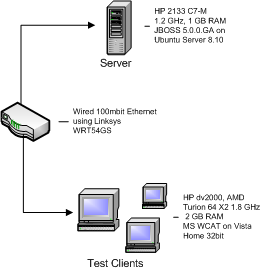
\includegraphics{Graphics/PTE.png}}
\caption{Testing Environment}
\label{fig:4.1}
\end{figure}


\section{Scope}

Our tasks include:
\begin{itemize}
 \item Carry out functional testing and report on any agressive memory leaks and exception occurences;
  \item Load test the application under for a range of typical user loads, measure both client and server side metrics (including garbage collection);
 \item Stress test the application, and identify the threshold where acceptable performance is not attained;
 \item Identify the best stress-resistant configuration;
 \item Carry out optimisation of the JVM, Application Server, and other parameters to improve run-time performance of the application;
 \item Construct three model that closely match the perfromance of observed results.
\end{itemize}

\begin{figure}[h]
% 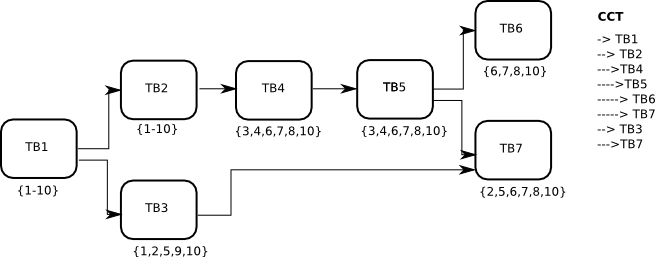
\includegraphics[bb=0 0 524 206]{Graphics/bean_diagram.png}
\scalebox{0.65}{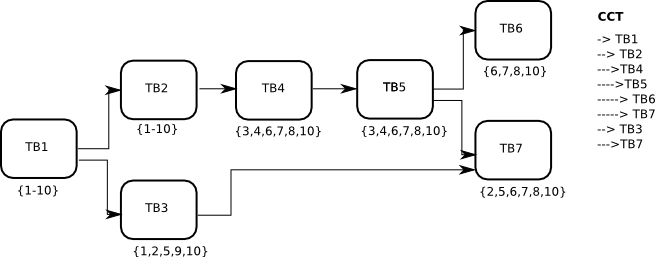
\includegraphics[bb=0 0 524 206]{Graphics/bean_diagram.png}}
 \caption{Bean calling sequence for config1...config10}
 \label{fig_bean_calling}
\end{figure}



\chapter{Plan}
In conjuction with the guidence notes given with the assignment we plan to divide the task into the sections below.

\section{Functional Testing}
For each configuration carry out functional tests to identify and quantify the following:
\begin{itemize}
\item memory leaks;
\item run-time exceptions.
\end{itemize}
From this testing we may also get some baseline measurements to feed into performance testing.

\section{Performance Testing}
Firstly we will define acceptable performance for the application in the form of a set of key performance scenarios. We will then carry out load testing to quantify the application performance under a range of loads. Following this stress testing will identify upper bounds for the application i.e. the maximum load within acceptable performance or to failure. We will profile performance by measuring standard system metrics: CPU activity; memory usage (both garbage collection performance and native memory utilisation); and network load. Client side metrics will also be measured including throughput, and response time. To carry out these tests we will use automated performance testing tools.

\section{Optimising Performance}
Following analysis of bottle necks from the performance testing we will attempt to improve performance and quantify the improvement made by tuning the following parameters:
\begin{itemize}
 \item Java Virtual Machine (JVM);
 \item JBoss application server settings;
 \item Operating sytem settings.
\end{itemize}

We will assess the impact of optimisations individually and also in combination, culminating in a suggested optimal configuration for our key performance scenarios.

\section{Modelling and Simulation}
We will use the parameters we measured in the preceeding sections to construct a model of some of the application configurations. We will use our model to explain the results we observed and explain some of the more unexpected results. The model should reflect the real performance metrics observed for a range of users.

We will formulate a theoretical model to explain the results we observed, this will use queuing theory models. If time allows we will also obtain alternative analysis with another method such as Petri Nets.


\chapter{Functional testing}

\section{Introduction}

Our first task is to check the functional correctness of the application. The functional tests to be carried out are:
\begin{enumerate}
 \item Check each application configuration for the occurence of Java exceptions;
 \item Check each application configuration for any aggressive memory leaks i.e. any leaks that would cause the JVM to run out of memory if the application was left running.
\end{enumerate}

Any configurations that exhibit any of the above behaviour\footnote{an application 'fault'} will be discounted from any further performance testing. As far as the black-box methods that are available to us allow, we will investigate the extent and location of the fault.

\section{Exceptions}

\subsection{Method}

To check for occurrence of Java exceptions in our application we set up our application with some added monitoring. We used a profiler tool\footnote{see appendices} that carried out instrumentation of specified classes (in our case those in package org.adaptivecellsj). The trace files produced by this tool gave us the calling sequence for these instrumented classes, enabling us to identify the bean that raised the exception (in conjunction with the diagram in figure \ref{fig_bean_calling}. From the AdaptiveCells/J documentation we know that each bean calls a method, 'simulateBusinessLogic', we can see during which particular call to this method the exception is raised, thus identifying the bean e.g. if for config1 the exception is raised in the second call to simulateBusinessLogic then the bean that raised the exception is TB2.

We invoked each configuration, in sequence, through the web page front end, accessible at url http://localhost:8080/adaptivecellsj/start.html. If an exception was raised we examined the JBoss log, and the trace file produced by the profiling tool.

\subsection{Results}

We established that three configurations raised exceptions\footnote{all of type java.lang.RuntimeException} config4, config5. Nothing of note was observed in the JBoss logs. Examination of the trace files showed that the following:

\begin{center}
\begin{tabular}{| c | c |}
 \hline
 Config & Bean raising exception \\
 \hline
 config4 & TB5 \\
 config5 & TB4 \\
 \hline
\end{tabular}
\end{center}

We repeated the test to check our results, which confirmed our initial findings. We can now discount config4, config5 from further testing.

\section{Memory Leaks}

\subsection{Method}

Despite Java having garbage collection memory leaks can still occur, primarily where an object is put into a long lived collection and not taken out once the object is no longer required.

The instructions for the assignment state that we identify aggressive memory leaks and remove them from further investigation. For our purposes we define an aggressive memory leak as one that would result in heap exhaustion within standard use of the application i.e. the memory is not freed by garbage collection.

We know from the AdaptiveCells/J documentation that memory leaks are implemented by allocating an array of bytes. Any aggressive memory leak should be visible as a large block of memory that isn't freed after a garbage collection. To identify configurations with aggressive memory leaks we used the following method:

\begin{enumerate}
 \item Monitor the application with JConsole;
 \item Using JMeter to create workload for 100 users access to AdaptiveCells/J at the same time;
 \item Setting up the loopcount in JMeter is forever in 60 minutes;
 \item Invoke the AdaptiveCells/J configuration that we are currently investigating, and then take a snapshot of memory usage;
\end{enumerate}

The above method was repeated for each of the configurations that did not cause Java exceptions to be raised. An aggressive memory leak should be evident from observing a steady increase in the memory allocated to byte arrays and that this allocation should not significantly decrease following the forced garbage collection.

\subsection{Results}

After testing each configuration for one hour, we found three configs cause memory leak including: config1, config2, and config9. Normally, garbage collection mechanism of Java will collect memory of system after used. The graph of the used memory continually fluctuated in the operation time of the system. Figure \ref{config3} showed the normal operation of the system. 

\begin{figure}[ht]
 \centering
 \scalebox{0.45}{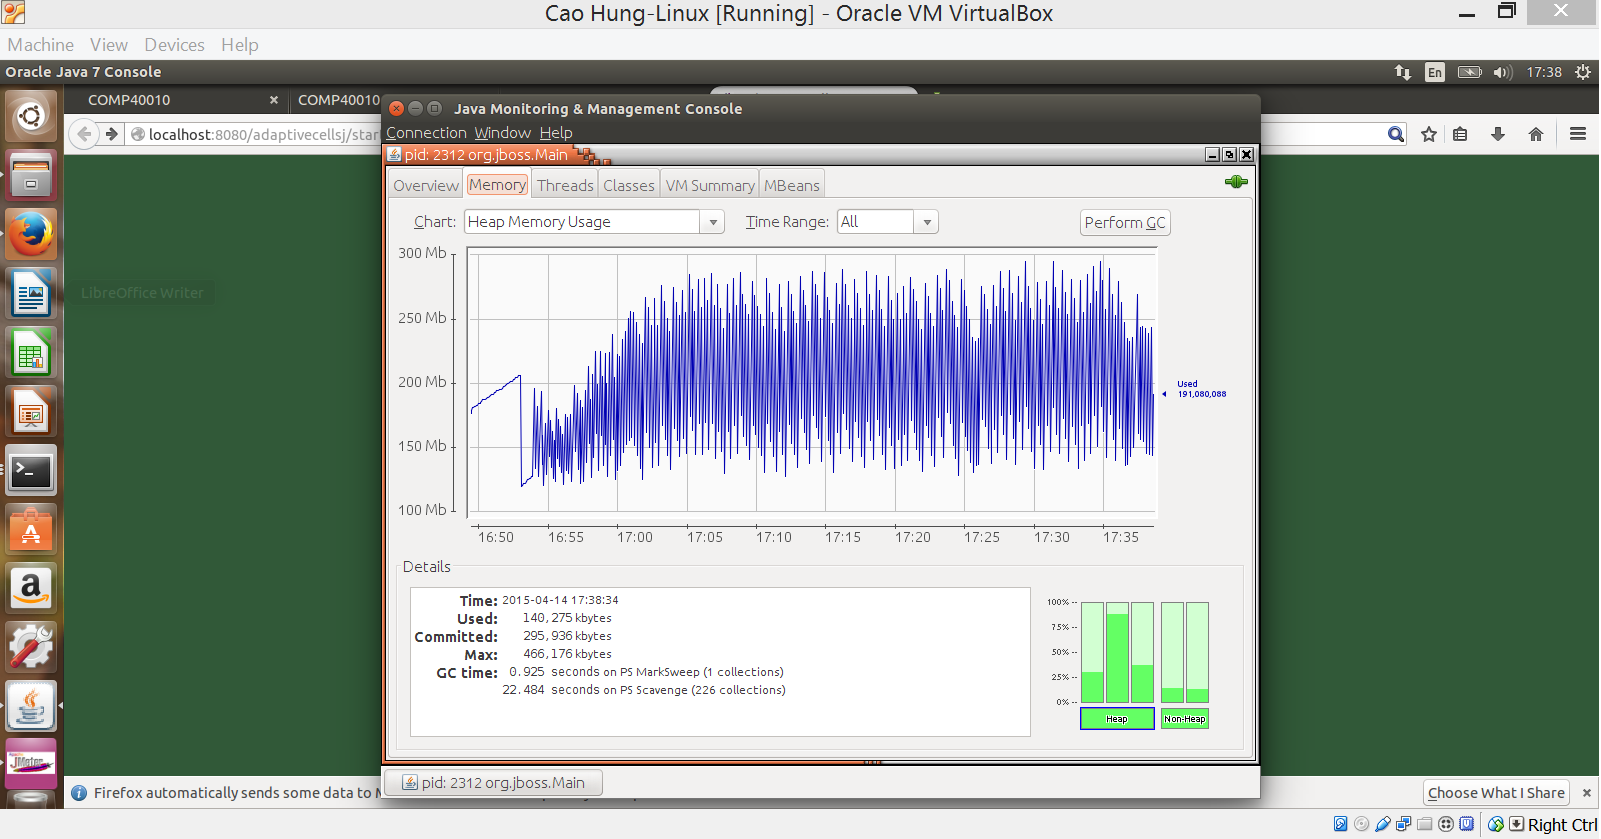
\includegraphics{Graphics/config3.png}}
 % func_memory_leaks.png: 638x448 pixel, 72dpi, 22.51x15.80 cm, bb=0 0 638 448
 \caption{Graph showing normal work of config 3}
 \label{config3}
\end{figure}

However, when memory leak occur in the system, the garbage collection mechanism could not free all memory and some spaces of memory was still occupied. After a certain time, the memory leak climbed higher and higher until the system absolutely crashed. An example of this case was indicated in Figure  \ref{config2}.

\begin{figure}[ht]
 \centering
 \scalebox{0.5}{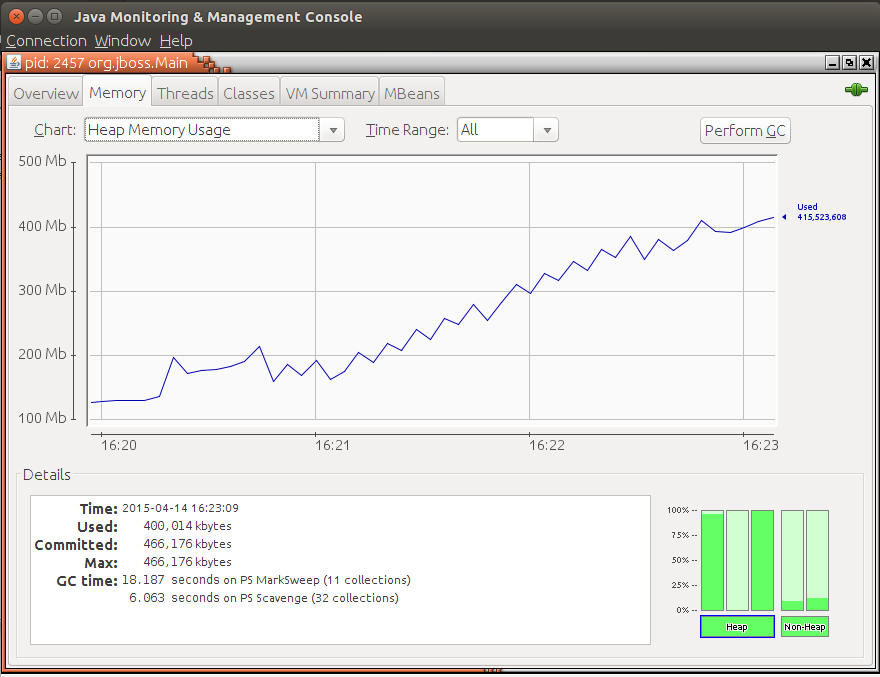
\includegraphics{Graphics/config2.png}}
 % func_memory_leaks.png: 638x448 pixel, 72dpi, 22.51x15.80 cm, bb=0 0 638 448
 \caption{Graph showing memory leak situation was caused by config 2}
 \label{config2}
\end{figure}

We established that two configurations had aggressive memory leaks, config1, config2 and config9. Table \ref{func_mem_leak_table} shows the data obtained.

\begin{figure}[h]
 \centering
\begin{tabular}{| c | c | c | c |}
 \hline
  & \multicolumn{3}{|c|}{Config} \\ \cline{2-4}
 Stage & config1 & config2 & config9\\
 \hline
 before running & 120,703,904 & 125,034,504 & 125,034,504 \\
 after collapse & 410,528,952 & 415,523,608 & 415,565,984 \\
 \hline
\end{tabular}
 \caption{Change in memory (from initial reading) allocated to byte[]}
 \label{func_mem_leak_table}
\end{figure}

Figure \ref{config2_2} indicated the error when the system collapse by the memory leak.

\begin{figure}[ht]
 \centering
 \scalebox{0.45}{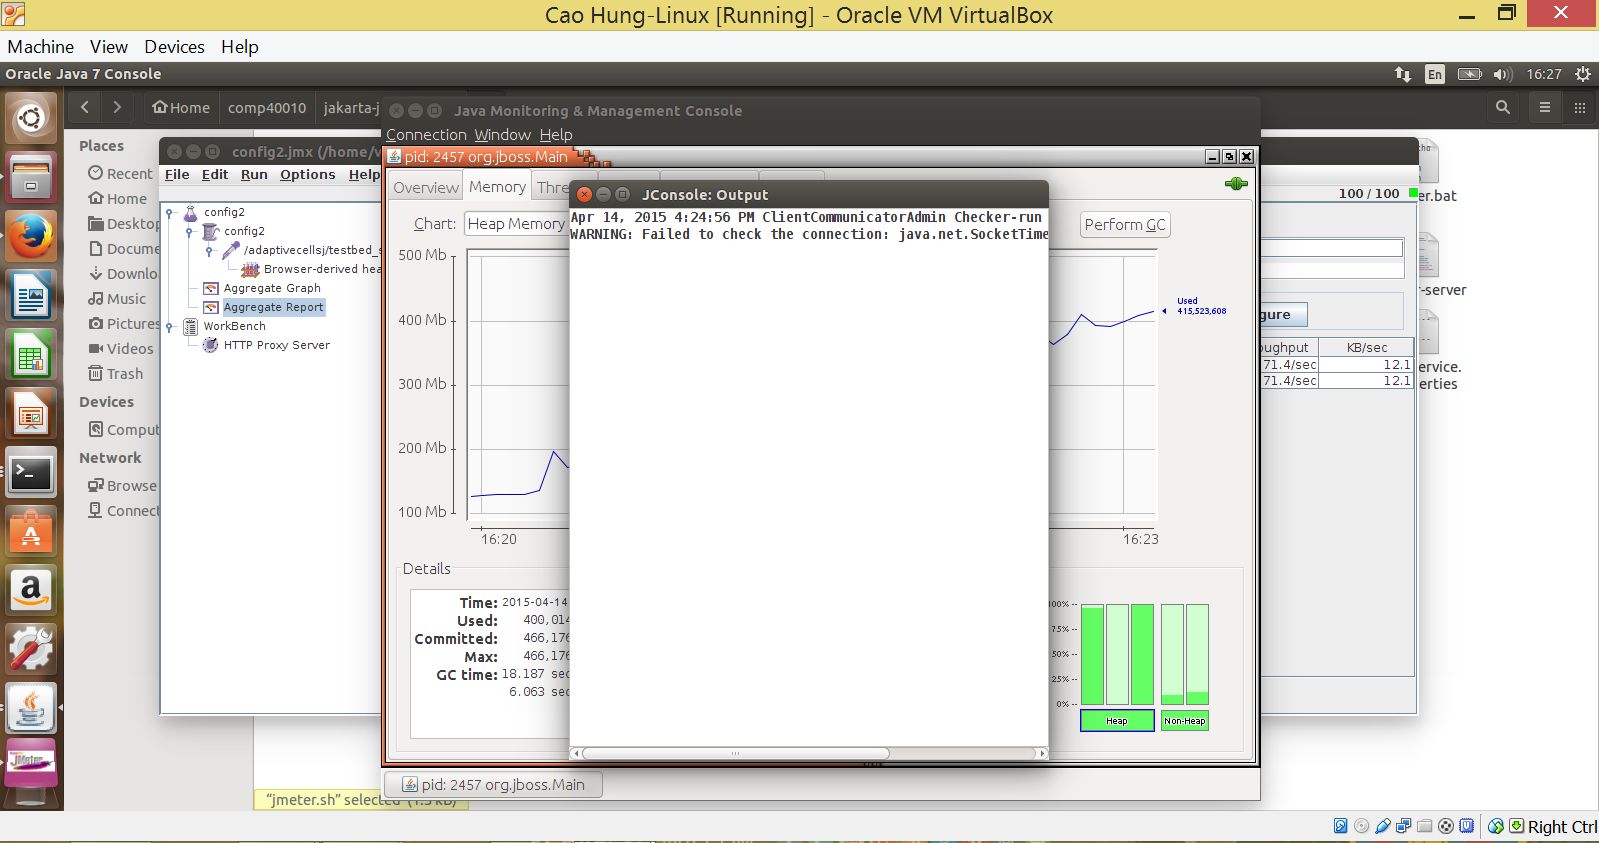
\includegraphics{Graphics/config2_2.png}}
 % func_memory_leaks.png: 638x448 pixel, 72dpi, 22.51x15.80 cm, bb=0 0 638 448
 \caption{Error when memory leakage happened}
 \label{config2_2}
\end{figure}

\section{Summary}

Following our functional testing we can discount config1, config2, and config9 because of agressive memory leaks and config4, config5 because of raising Java exceptions. This leaves config3, config6, config7, config8, and config10 remaining to carry out performance analysis on.

\chapter{Load Testing}

The purpose of load testing is to determine the ability of the application to perform during the key performance scenarios that we outlined in section 1.3. 


\section{Measurements}
In order to evaluate the ability of the application to meet its target we must use monitors that can measure the applications response time. As the HTTP responses do not contain client-side scripts or CSS we can measure response time as time to last byte (TTLB) of the HTML page. As well as measuring the average TTLB we must also measure the percentage of responses that are within the SLA as a large standard deviation may hide an unexpected number of failures within the average TTLB.

\section{Test Setup}
In order to simulate the expected user load we created a test using four different transactions. The transactions vary by the use of HTTP 1.0 and HTTP 1.1 with keep-alive TCP connections and the length of the "Think Time" between requests.

\begin{center}
\begin{tabular}{|l | c | c | c | c |}
\hline
ID & Weight & Think Time & HTTP & Keep-alive \\
\hline
1 & 10 & 300 & 1.0 & No \\ 
2 & 10 & 400 & 1.0 & No \\ 
3 & 40 & 300 & 1.1 & Yes \\ 
4 & 40 & 400 & 1.1 & Yes \\
    \hline
\end{tabular}
\end{center}

Microsoft's Web Capacity Analysis Tool (WCAT) was used as the primary testing software. The results where verified with a number of spot checks using JMeter. 

\begin{center}
\begin{tabular}{| c | c | c | c |}
\hline
Virtual Clients & Ramp up & Duration & Cool Down \\
\hline
150 & 300 & 600 & 60 \\ 
500 & 300 & 600 & 60 \\ 
1000 & 300 & 600 & 60 \\ 
\hline
\end{tabular}
\end{center}

Before each test the Jboss server is restarted and a warm-up test was is carried out with the following settings. 
\begin{center}
\begin{tabular}{| c | c | c | c |}
\hline
Virtual Clients & Ramp up & Duration & Cool Down \\
\hline
20 & 40 & 300 & 20 \\ 
\hline
\end{tabular}
\end{center}

\section{Results}
We carried out load testing in order to get a baseline of system performance in regard to our key performance scenarios. We looked at both client-side and server-side measures. 
\subsection*{Throughput} 
The throughput for the overall test is measured to determine the number of transactions the application can complete within each given time.

\begin{figure}[h]
\centering
\scalebox{0.65}{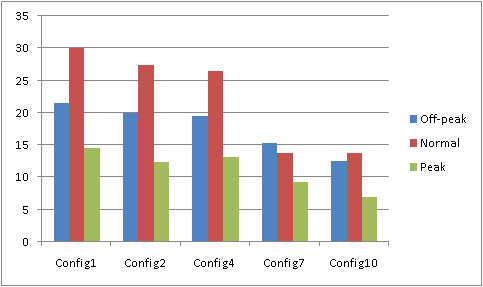
\includegraphics{Graphics/Throughput2.png}}
\caption{Throughput - requests per second}
\label{fig:4.2}
\end{figure}

We conclude from the results that the off-peak load does not burden the system and that the maximum throughput is reached after the off-peak load but before the high peak load. The system slows quickly as it nears the high load and we can assume that one or more of the system resources are under strain.

\subsection*{Average Response Times} 
Generally, as the page sizes are very small and the response is delivered in one HTTP packet, the time to last byte and the time to first byte will be equal.

\begin{figure}[h]
\centering
\scalebox{0.65}{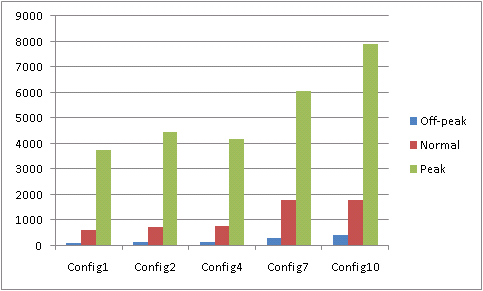
\includegraphics{Graphics/ResponseTimes2.png}}
\caption{Response Times - Time to Last Byte in Milliseconds}
\label{fig:4.3}
\end{figure}

The average response time of each of the configs for each of the loads meet the performance objective. We can see the different characteristics of each of the configs. While each of the configs shows variations in their response times on each load, there is common pattern shown in the changes to response times as the loads increase. 

\subsection*{Response Times Within 8 Seconds}
As we have a defined a maximum response time we must be careful not to just use averages in measuring the response time of the system as it does not tell us how many responses where actually outside our target. For this we measure the percentage of responses within the target.


\begin{figure}[h]
\centering
\scalebox{0.65}{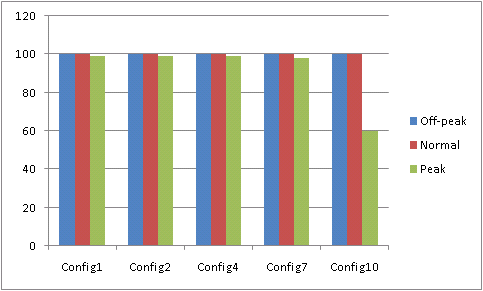
\includegraphics{Graphics/PercentWithinSLA.png}}
\caption{Percentage of responses within 8 seconds}
\label{fig:4.4}
\end{figure}

While the average response times are within the target we can see that the not all of the responses where within the target. The number of request outside the target for configs 1, 2, 4 and 7 are small however for config 10 only 60 percent of responses within 8 seconds. This is a serious problem that could stop the project from going live.


\subsection*{Errors}
Any errors returned by the server are also measured. We check the server logs for any errors that were not reported to the client. 
During the testing of the configs, on each of the different loads, no errors were recorded.



\subsection*{Resources}
We also made spot checks on the usage of server and network resources during the load test to gain a picture of the characteristics of applications. We saw that in all the tests CPU utilization was very high while memory and network usage was low. We use these measurements as inputs into our initial stress test plan. 







\chapter{Stress Testing}
The purpose of the stress test is to observe how the system behaves as we steadily increase its load beyond the maximum number of users defined in the key performance scenarios. 

\section{Measurements}
We are interested to know whether the system will crash or if there will be a steady decline in response times. We are also interested in how the system recovers from an unusually high load; can the response times observed in our initial normal load test be replicated after the stress test without restarting the system? To answer these questions we measure throughput and average response times. We also measure errors and HTTP response codes.

\section{Test Setup}

\subsection{Increase Load}
To simulate stress on the system we created a series of tests which steadily increase the load on the server. We used the same mix of transactions used for load testing. The following set of tests were carried out for each the configs.


\begin{center}
\begin{tabular}{| c | c | c | c |}
\hline
Virtual Clients & Ramp up & Duration & Cool Down \\
\hline
20 & 300 & 300 & 60 \\ 
50 & 300 & 300 & 60 \\ 
80 & 300 & 300 & 60 \\ 
100 & 300 & 300 & 60 \\ 
150 & 300 & 300 & 60 \\
200 & 300 & 300 & 60 \\ 
300 & 300 & 300 & 60 \\ 
400 & 300 & 300 & 60 \\ 
. &  &  & \\ 
. &  &  & \\ 
2000 & 300 & 300 & 60 \\ 
\hline
\end{tabular}
\end{center}

The Jboss server was restarted only at the beginning of each series and not in between each test as had been the case with the load tests.


\subsection{Recovery}
In order to see how the system recovers we compare the results of our standard load test with a normal amount of users as defined in the key performance scenarios against the same test carried out after the system has experienced an exceptional high load.

\begin{center}
\begin{tabular}{| c | c | c | c |}
\hline
Virtual Clients & Ramp up & Duration & Cool Down \\
\hline 
2000 & 300 & 300 & 60 \\ 
500 & 300 & 600 & 60 \\ 
\hline
\end{tabular}
\end{center}

\section{Results}


\subsection*{Throughput} 
The throughput for the overall test is measured to determine the number of transactions the application can complete within each given time.


\begin{figure}[h]
\centering
\scalebox{0.65}{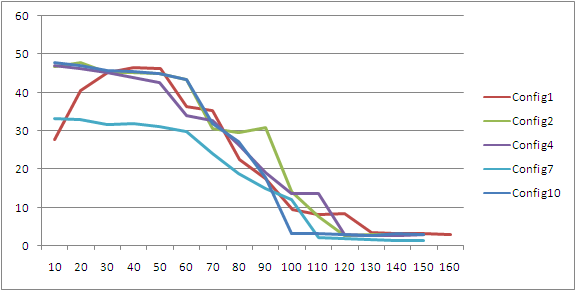
\includegraphics{Graphics/StressThroughput.png}}
\caption{Throughput under stress}
\label{fig:5.1}
\end{figure}

From the throughput test we see that after the maximum work rate is reached the system slowly declines as the load increases. At a certain point the decline stops and the steady state remains until a point when the server starts to refuse connections. 


\subsection*{Average Response Times} 
Generally, as the page sizes are very small and the response is delivered in one HTTP packet, the time to last byte and the time to first byte will be equal.

\begin{figure}[h]
\centering
\scalebox{0.65}{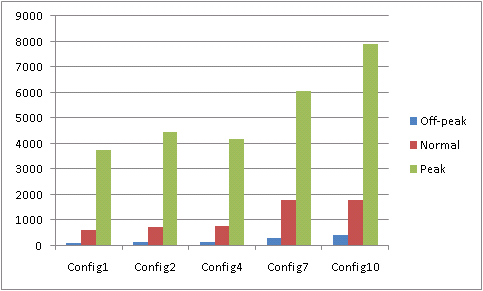
\includegraphics{Graphics/ResponseTimes2.png}}
\caption{Response Times - Time to Last Byte in Milliseconds}
\label{fig:5.3}
\end{figure}

The average response time slowly declines as the load increases. At a certain point the decline stops and the steady state remains as the server starts to refuse connections.


\subsection*{Recovery} 

\begin{figure}[h]
\centering
\scalebox{0.65}{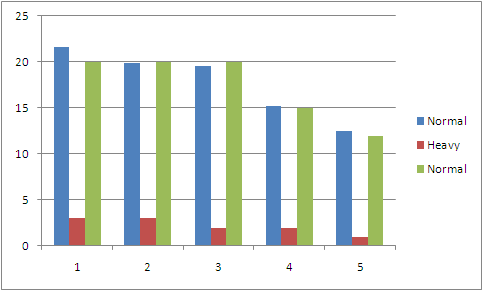
\includegraphics{Graphics/Recovery.png}}
\caption{System recovery from abnormal high load}
\label{fig:5.2}
\end{figure}

From these tests we observe that the systems ability to recover and continue to effectually service request at normal loads is not affected by the abnormally high load.


\subsection*{Errors} 
As the number of virtual clients is increased requests to the server are rejected. The following graph displays the percentage of rejected requests for each of the tests.

\begin{figure}[h]
\centering
\scalebox{0.65}{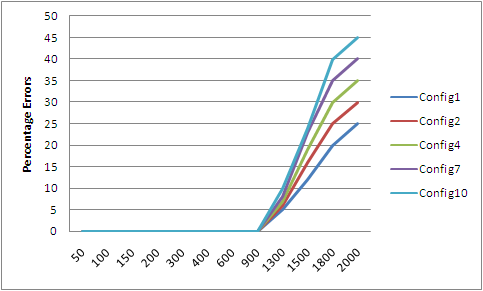
\includegraphics{Graphics/PercentageErrors.png}}
\caption{Percentage of responses containing errors}
\label{fig:5.3}
\end{figure}

\subsection*{Resource usage} 
During the tests we make a number of spot checks on the system resources.  We obsevered that the CPU was at maximum utilization.  Memory and Network resources where not under strain.  There where a number of TCP packets dropped due to the maximum utilization of the TCP buffer. 



\chapter{Optimisation}

\section{Introduction}

The tests carried out during our load and stress testing were carried out on a server with an 'out of the box' configuration i.e. no changes were made to the default configuration. Similarly, the operating system was not optimised. In this section we aim to optimally configure the application for performance. 

We will specifically look at the following parameters:
\begin{itemize}
 \item Application server settings;
 \item Java Virtual Machine settings;
 \item Operating system settings;
\end{itemize}

When trying to optimise for performance we classify improvements by:
\begin{enumerate}
 \item Improving application performance for a constant load i.e. minimising response time for a given load and throughput;
 \item Maximising throughtput, keeping an acceptable response time i.e. increasing the number of users the application will support with an acceptable response\footnote{An extension to this improvement is to check for improved stress testing response.}
\end{enumerate}

We will focus on both aspects in optimising performance for AdaptiveCellsJ.

\section{Methodology}

In the optimisation process we will adhere to the following principles:
\begin{itemize}
 \item Only change one parameter at a time so as to isolate it;
 \item Carry out a a before and after test, measuring throughput, and response time on the client, and monitoring server parameters of CPU utilisation, network bandwidth utilisation, and JVM memory/heap utilisation (in tests involving memory);
 \item Ensure that the original load is high enough to adequetly stress the server (using monitoring tools and some adjustment as required);
 \item Allow the test to run for long enough to reach a steady state (at least ten minutes);
 \item Ensure uniformity for each test by restarting the application each time.
\end{itemize}

In testing we will follow the following general process:
\begin{enumerate}
 \item Carry out our base-line test on a pre-determined configuration i.e. with no changes from the defaults;
 \item Pick a client load that stresses the server adequetly - we will asses and adjust this by carrying out server monitoring;
 \item Carry out the optimisation and restart the application server;
 \item Carry out the test at the same client load as before the optimisation;
 \item Compare the throughput, and response time for the before and after configurations.
\end{enumerate}

\subsection*{Software and hardware environment}

We picked a test environment that had a powerful client machines, and a low specification server machine. This configuration was chosen so that client overloading would not occur.\footnote{As this would give erronous results.} During out tests the client machine was monitored and average CPU utilisation was well below 25\%. The client software, JMeter, was also monitored for heap usage, which also was well below the heap allocated (512MB).

We used JBOSS 4.0.4 (with JBOSS profiler installed), with Java 1.5.0 HotSpot. Client load was simulated with JMeter.v2.3.2.

\begin{figure}[ht]
 \centering
\begin{tabular}{| c | c | c |}
 \hline
  & \textbf{Client} & \textbf{Server} \\
 \hline
 \textbf{Operating system} & Open Suse 10.3 (64 bit) & Open Suse 10.3 (32 bit) \\
 \textbf{Memory} & 4GB & 1GB \\
 \textbf{Processor} & Intel Core 2 Duo (Quad core) @ 2.66 GHz & Intel P4 @ 2.8 GHz \\
 \hline
\end{tabular}
\caption{environment used}
\end{figure}

The network between the two machines was 100Mbit wired ethernet, using a ZyXEL P-660HW router.

\section{Optimisations}

\subsection*{Baseline Response}

To obtain a baseline measure of how this configuration responded under load we carried out some initial tests using the, 'out of the box', configuration. The first observation we made was that the default settings were possibly set too high for our hardware setup. Many authors recognise that setting parameters, such as thread pool sizes too high is a performance anti-pattern\cite{performance_solutions}. Initial monitoring indicated that the thread pool setting of 250 threads (for the embedded web container), was possibly too high. For the many of the parameters that are widely recognised to have the largest impact on performance require that the number of clients is larger than the thread pool\cite{model_server_settings_jee}. If this were not the case it would be very hard to measure as the top value of the parameter would have little to no impace. We found that at over 250 user the server processor utilisation was over 99\%. 

To find out the response of this setup we carried out the following test:
\begin{enumerate}
 \item Set the thread pool to 10, and the web container queue size to 40\footnote{carried out by editing values in server.xml file};
 \item Monitored the throughtput and response time for a range of clients;
 \item Observed with the point where throughput improvement started to fall off, and response time increased.
\end{enumerate}

Our JMeter test was structured so that we also tested fetching the initial static page (and embedded images), as well as submitting it. This was to ensure that we were testing all aspects of the application and stressing components of the JBOSS application server that the parameters may impact. We measured the total throughput i.e. the total number of served requests (number of times each web page element is served + number of submits of the page). We used config10 for this test as it is the most processor intensive of the configurations\footnote{see table in appendices}.
\newline

\begin{figure}[ht]
 \centering
 \scalebox{0.5}{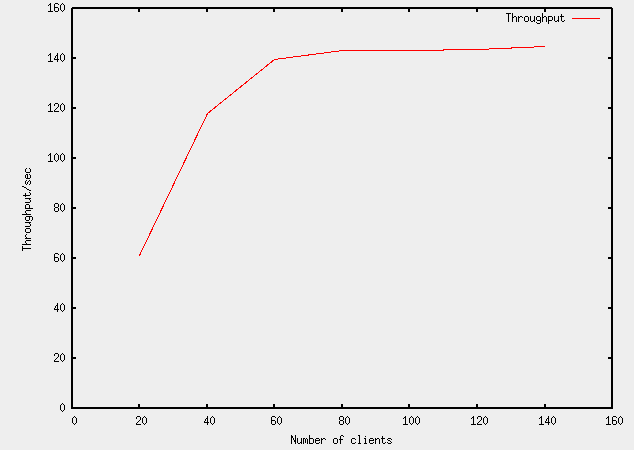
\includegraphics{Graphics/optimise_gen_response_tp.png}}
 \caption{Throughtput for a range of clients}
 \label{graph_response_tp}
\end{figure}

\begin{figure}[ht]
 \centering
 \scalebox{0.5}{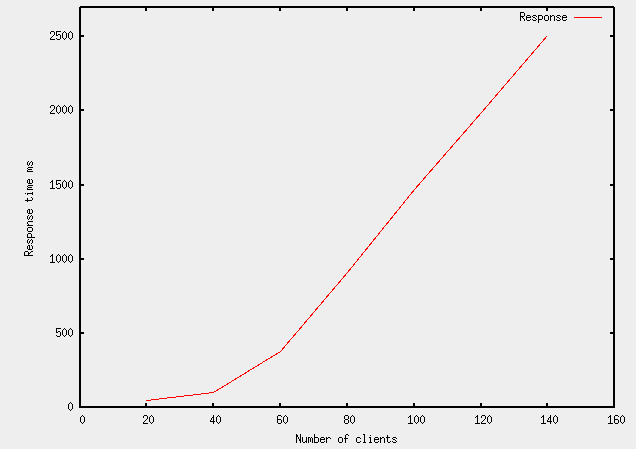
\includegraphics{Graphics/optimise_gen_response_rt.png}}
 \caption{Response time for a range of clients}
 \label{graph_response_rt}
\end{figure}

As the graphs in figures \ref{graph_response_tp} and \ref{graph_response_rt} show, we get a noticable drop in performance at 60 users. This is for the setting of 10 threads for the embedded web container, with a queue of 40. We will use this as a baseline figure. During our tests we measured server performance, CPU usage rose gradually as we increased the number of clients, but never rose above 90\%. Memory usage by the application was consistantly low. Both these indicate that this range of clients should give reliable, repeatable results and that we are not hitting hardware limits e.g. CPU, or memory. We will use this configuration as our baseline during the optimisation process.

\subsection*{Thread Pool Settings}

\subsubsection*{Embeded Web Container}

As identified in earlier the default settings for the embeded web container are two high for our environment. This results in maxing out the CPU as we increase the number of clients. For the purpose of establishing our base line configuration we greatly reduced our the number of threads and the queue size for the embeded web container (EWC), to 10 threads and a queue of 40 requests. Other work has been done into how these two parameters impact performance\cite{model_server_settings_jee}, concluding that these parameters significantly impact performance. During the baseline tests we monitored the counter 'currentThreadsBusy', provided by the JMX bean jboss.web. We observed that this parameter quickly rose to 10, indicating that all 10 threads in the pool were working. Articles indicate that the number of threads used should be less than 70\%-80\% of the maxThreads value (in our case 10)\cite{master_the_boss}. 

We will investigate the effect of increasing the thread pool size and the queue size. In our baseline tests we did not receive any request timeout responses. We should have received this error if a request arrived when the queue was full. This theory was backed up by our test. We increased the queue size by from 40 to 100, which made little to no difference to our results (less than 1\% deviation from the baseline measure). For a thread pool of 10 this queue size would seem to be sufficient.

Moving on to investigate the effect of increasing the web container threadpool setting. Using the guideline above we picked a thread pool size of 100 threads, if the processor did not max out when the currentBusyThreads values was close to 100, we would increase this. We re-ran the baseline tests, but with the thread pool set to 100.

\begin{figure}[ht]
 \centering
 \scalebox{0.5}{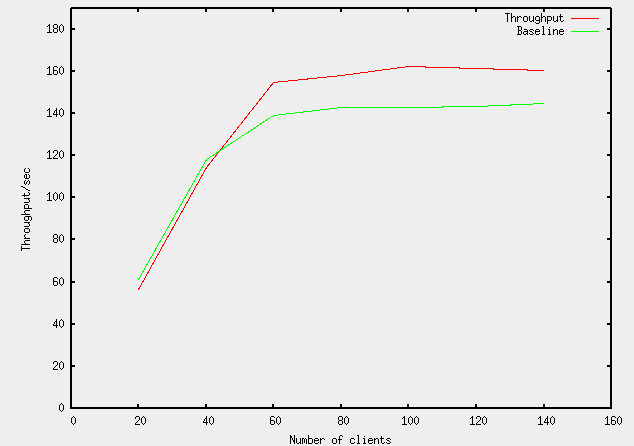
\includegraphics{Graphics/wc_throughput_thread_pool_tp.png}}
 \caption{Throughput baseline compared to larger thread pool.}
 \label{graph_tp_tput}
\end{figure}

\begin{figure}[ht]
 \centering
 \scalebox{0.5}{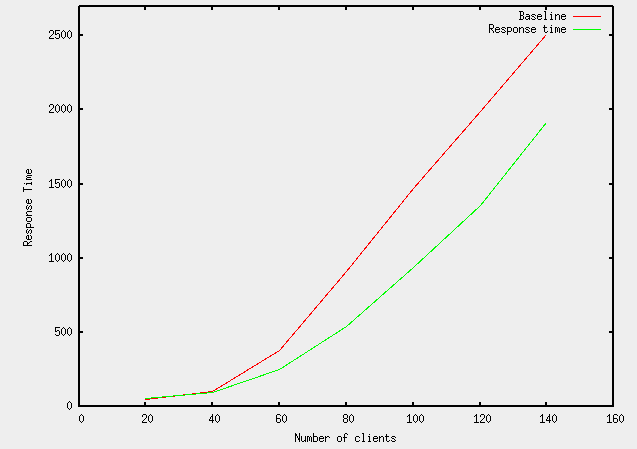
\includegraphics{Graphics/wc_response_thread_pool_tp1.png}}
 \caption{Response time, baseline compared to larger thread pool.}
 \label{graph_tp_rt}
\end{figure}

As the graphs in figures \ref{graph_tp_tput}, and \ref{graph_tp_rt} indicate, performance did improve with the new thread pool setting. Both throughput and response time showed improvements. Comparing the throughput to the baseline response, we see that the drop off occurs later (at 60 clients, compared to 40 clients), giving a ceiling that is higher by approximately 20 requests/second. We noted that at around 120 clients the the server processor was operating at nearly 100\%, indicating that we were at saturation of this resource and that this is probably a hardware limit. Maximum throughput would be governed, in this case, by the CPU resouce, and is given by 1/S (mean service time) \cite{model_server_settings_jee}\cite{performance_solutions}. In our case the system would be modelled by a closed queueing network model\footnote{this will be discussed more fully in the modelling section.}, for this model the arrival rate is state dependent as if we have K clients, but there are k jobs at the server (waiting for service) then there are only K-k clients that can send in new requests\cite{model_server_settings_jee}. If the system is using all the threads in the web container, then any new requests will be queued (i.e. giving a bigger queue). This means that k will be higher in our baseline case, than for a system with more threads in the pool. As \begin{math}\lambda_{k} \propto (K-k)\end{math} - where \begin{math}\lambda_{k}\end{math} is arrival rate for kth request\cite{model_server_settings_jee}, then this would explain our higher throughput.

The results for response time also showed significant improvement, we note that up to 120 clients the improvement increased with number of clients (at which point we reached CPU saturation). This also makes sense as response time = queue residence time + service time, increasing the number of threads would decrease the queue residence time, and hence decrease response time. 

This test would show that a value of around 100 threads, and a queue size of 40 is sufficient optimisation to improve performance up to around 120 clients. Above this demand we seem to be hitting processor saturation.

\subsubsection*{JBOSS Thread Pool}

Once the embeded web container has dealt with the request it must be passed onto the EJB tier. As shown in figure \ref{fig_bean_calling}, this tier calls a number of beans (depening on the configuration). These requests are carried out by a thread pool, in which the queue size and number of threads is configurable in a similar manner to the embedded web container. The parameters are specified in the file jboss-service.xml. We left the queue size at the default of 1,000 and altered the MaxPoolSize parameter (default is 10 threads). During our tests we monitored the queueSize measure in the jboss.system JMX bean, the guideline\cite{master_the_boss} is that if the queueSize approaches the MaxThreadPool size then you may need more threads (if the system is not at CPU/Memory saturation). We kept the number of clients at 60, and we used the configuration in set for the web container (100 threads, queue of 40), rather than the base line configuration. This was chosen because we wanted to avoid CPU saturation, hence the 60 clients, but balanced against this we wanted to maximise the rate that requests reached the EJB tier. Through trial and error we established that a load level of 60 clients provided adequete load without saturation.

We ran our test, with different numbers for MaxThreadPool (1, 5, 10, 15, 20, 25). We encoutered some unusual results. Firstly the queueSize was always 0, except for the case of having 1 thread in the pool, in which case the queueSize was always 1. This seems unusual, and unexplainable at the moment. Secondly changing the MaximumPoolSize parameter had no effect on throughput or response times (less than 4\% deviation). We tried changing other parameters (e.g. BlockingMode), but this made no difference. Further investigation would be required to understand what was happening here. For the queue length to be 1 then by Little's law RT = (1/throughput) - we will investigate this in the modelling section.

\subsection*{Garbage Collection and Memory Usage}

We monitored the JVM heap usage and garbage collection by using the -xloggc flag. The resulting log file was analysed with gcviewer. We observed the results indicated below (before row). The throughput was already quite good, at 99.34\%, but the application pauses was perhaps a little poor at 4.05s. We increased the heapsize, setting the minimum and maximum to the same value of 512m. We also changed the heap ratio, giving the young generation 25\% of the heap. This was done because for this application we know that the beans are stateless and that each bean frees up it's memory allocated fairly soon. This was also shown to be true by looking at the graph of heap usage, the application allocates it's memory and frees it shortly afterwards. The trace also backed this up by showing only 10\% of the tenured generation was used, but 50\% of the young generation was used.

As shown in figure \ref{gc_performance} we made a small improvement in throughput, and a large improvement in pauses (owing to fewer garbage collections). This performance seemed adequate, and confirms our theory that garbage collection is not a big factor for this application, even with the default settings.

\begin{figure}[h]
 \centering
\begin{tabular}{| c | c | c |}
 \hline
  & Throughput & Acc pauses\\
 \hline
 Before change & 99.34\% & 4.05s \\
 After change 5 & 99.75\% & 1.3s \\
 \hline
\end{tabular}
 \caption{Garbage collection performance}
 \label{gc_performance}
\end{figure}

\subsection*{Other possible areas for optimisation}

After analysing results from our load and stress testing, and also the results of the optimisations. We observed that for this appliction after optimisation, the biggest bottle neck is CPU saturation. 

There are a number of other areas we could optimise (given the time), but we feel that these areas would produce diminishing returns. The areas are:

\begin{itemize}
 \item Operating system settings (network settings, memory);
 \item Slim down JBOSS (set production settings e.g. turn of JSP compilation, remove surplus services e.g. mail, log4j);
 \item Tune pool size (we know that our beans are stateless session beans, we could look at the object pool size).
\end{itemize}

\section{Summary}

Our optimisations have given a significant improvement in throughput and response time, within the capacity of our test environment. 


\chapter{Modelling}

\section{Introduction}

Up to this point we have been analysing the performance of the application by empirical measurement. This has yielded some good results and assisted us in optimising the application. Problems with this approach in isolation are:

\begin{enumerate}
 \item We may want to simulate use cases where we will not have the hardware necessary to support the test;
 \item We can get greater insight into what is happening in different parts of the system with a model - helping us identify bottlenecks and explain exceptional observed results.
\end{enumerate}

In this section we will contruct a model of the AdaptiveCells/J application, using a tool that models queueing networks called JMT. The structure of the model will come directly from the application structure. Model parameters will come from similar measurements that we made in previous sections. Once we have constructed the model we will compare the output of the model, under different loads, with the actual measured experience.

\section{Methodology}

For the purposes of building the model we will simplify our simulation used in the optimisation section and use a similar model to that used in the loading section. We will simplify by eliminating the process of obtaining the static pages, and just go straight to the part that submits the config chosen to the application.
The model we will contruct will be based on the structure of the JBOSS application\footnote{see appendices} with the following characteristics:

\begin{itemize}
 \item a server node representing the Tomcat embedded webserver, with a queue size and number of servers taken from the JBOSS configuration;
 \item a server node representing the EJB tier with parameters taken from the observed values of tests;
 \item the model will be closed, as this more closely matches the use cases we are working with - a fixed number of users submitting a request, thinking and then submitting another request.
\end{itemize}

The modelling tool allows us the set the size of queues, the number of servers (corresponding to thread pools), and service time of each node. 


% appendicies
\appendix

\chapter{AdaptiveCells/J}

\section*{Overview of AdaptiveCells/J}
AdaptiveCells/J is a J2EE, open source\footnote{download from http://www.adaptivecellsj.sourceforge.net}, benchmarking system, allowing development of an artificial testbed without creating code. For the purposes of this project we were using the the application for performance testing of our application in different contexts.

AdaptiveCells/J test-beds allow specification of precisely timed faults to occur, with behaviour fully configurable at runtime by selecting a configuration. The following behaviour can be replicated:

\begin{itemize}
\item CPU usage behaviour;
\item memory allocation;
\item memory leaks;
\item raising exceptions.
\end{itemize}

\section*{Description}
The AdaptiveCells/J framework consists of structurally identical EJBs, that are customised by a deployment descriptor. The deployment descriptor specifies values for key parameters:
\begin{itemize}
 \item CPU overhead (integer value of the number of repetitions that a pseudo random number is generated);
 \item Memory overhead (the size of byte arrary allocated when the EJB is called);
 \item Memory leak (size of the block to be allocated and leaked);
 \item Exception to be raised;
 \item First target EJB (the first EJB to call);
 \item Second target EJB (the second EJB to call);
\end{itemize}
These parameters configure the runtime behaviour and footprint of each bean. 

Each bean simulates a 'real' EJB by emulating load (CPU and memory), and calling other beans in a specified calling sequence. Each bean can have a number of configurations, each one optionally specifying values for the above parameters. Each configuration is identified by a configuration name. The same configuration name should be used for each bean participating in a particular calling sequence e.g. 'config1'. 

Each bean exposes a single method simulateBusinessLogic(), which takes the configuration name as a parameter. The bean will then read the parameters for that configuration and then generate the appropriate CPU and memory overhead, and then call the specified target EJBs.

\section*{Structure}
The application is comprised of: 
\begin{itemize}
 \item A presentation tier (a Servlet);
 \item A business logic tier (a number of Session Beans, with a set of configurations, each configureation specify one set of the above parameters for each bean).
\end{itemize}

The web front-end to the application is an html page, where the configuration to be tested is specified by the user, and a servlet. This configuration enables web-based stress and loading tools to be used to simulate sets of simultaneous users. The first bean that is called by the front end is, by convention, called TB1. Complicated calling sequences can be built up with the first target and second target parameters. There is no mechanism to support loops in the calling sequence.


\chapter{Configurations}

\section*{Overview}

Using tools such as the jmx-console we were able to gain further insight into the ten configurations of our application. The table below sumarises the bean parameters for each of the ten configurations:

\begin{center}
\begin{tabular}{| c | l | r | r | r | r | r | r |}
 \hline
 \multicolumn{2}{|c|}{} & \multicolumn{6}{|c|}{Bean} \\
 \hline
 Config & Parameter & TB1 & TB2 & TB3 & TB4 & TB5 & TB6 \\ \hline
 \multirow{3}{*}{1} & CPU & 1,000 & 2,000 & 3,000 & & &  \\
  & Memory & 100 & 200 & 300 & & & \\ 
  & Memory Leak & 10,000 & & & & & \\ \hline
 \multirow{3}{*}{2} & CPU & 1,000 & & 3,000 & & & 9,000 \\
  & Memory & 100 & & 300 & & & 900 \\ 
  & Memory Leak & 10,000 & & & & & \\ \hline
 \multirow{2}{*}{3} & CPU & 1,000 & 2,000 & & 5,000 & & \\
  & Memory & 100 & 200 & & 500 & & \\\hline
 \multirow{3}{*}{4} & CPU & 1,000 & & 3,000 & & 7,000 & \\
  & Memory & 100 & & 300 & & 700 & \\
  & Exception & & & & & Yes & \\ \hline
 \multirow{3}{*}{5} & CPU & 1,000 & 2,000 & & 5,000 & & \\
  & Memory & 100 & 200 & & 500 & & \\
  & Exception & & & & Yes & & \\ \hline
 \multirow{2}{*}{6} & CPU & 1,000 & 2,000 & 3,000 & 5,000 & 7,000 & 9,000 \\
  & Memory & 100 & 200 & 300 & 500 & 700 & 900 \\ \hline
 \multirow{2}{*}{7} & CPU & 1,000 & & 3,000 & & & 9,000 \\
  & Memory & 100 & & 300 & & & 900 \\ \hline
\multirow{2}{*}{8} & CPU & 1,000 & & 3,000 & & & 9,000 \\
  & Memory & 100 & & 300 & & & 900 \\ \hline
\multirow{3}{*}{9} & CPU & 1,000 & 2,000 & & 5,000 & &  \\
  & Memory & 100 & 200 & & 500 & & \\ 
  & Memory Leak & 10,000 & & & & & \\ \hline
 \multirow{2}{*}{10} & CPU & 1,000 & & 3,000 & & 7,000 & 9,000 \\
  & Memory & 100 & & 300 & & 700 & 900 \\ \hline
\end{tabular}
\end{center}






\chapter{JEE Application Structure}

\section*{Overview}
A brief overview of the components in the JBOSS implementation of the JEE specification is given below. 

!!! To finish

% bibliography using bibtex

\bibliographystyle{plain}
\bibliography{biblio}
\end{document}
